\clearpage

\section{Histograms on Consecutive INC1024 Runs~\label{sec:s9_1024_runs}} 
This section exhibits histograms on (three) consecutive runs of INC1024 via SEDONA. 
The detailed description of the base data is from Table~\ref{tab:exp_notes2}.

\begin{table}[h]
\begin{center}
\begin{tabular}{|p{2cm}|p{3cm}|p{3cm}|p{4cm}|p{3.5cm}|} \hline
Machine & Task Length (sec) & Description & Experiment Period & Relevant \linebreak Histograms\\ \hline
{\tt sodb9} &  INC1024 & 300 samples, each & 2017-04-12 $\sim$ 2017-04-23 & 
Figs.~\ref{fig:s9_inc1024_et} and~\ref{fig:s9_inc1024_pt}\\ \hline
\end{tabular}
\end{center}
\vspace{-.2in}
\caption{Notes on experiment runs used for histograms\label{tab:inc1024_run_notes}}
\end{table}

\clearpage
\newpage

\subsection{ET}

\begin{figure}[hp!]
	\centering
	\subfigure[ET frequency on INC1024-Run1]{
		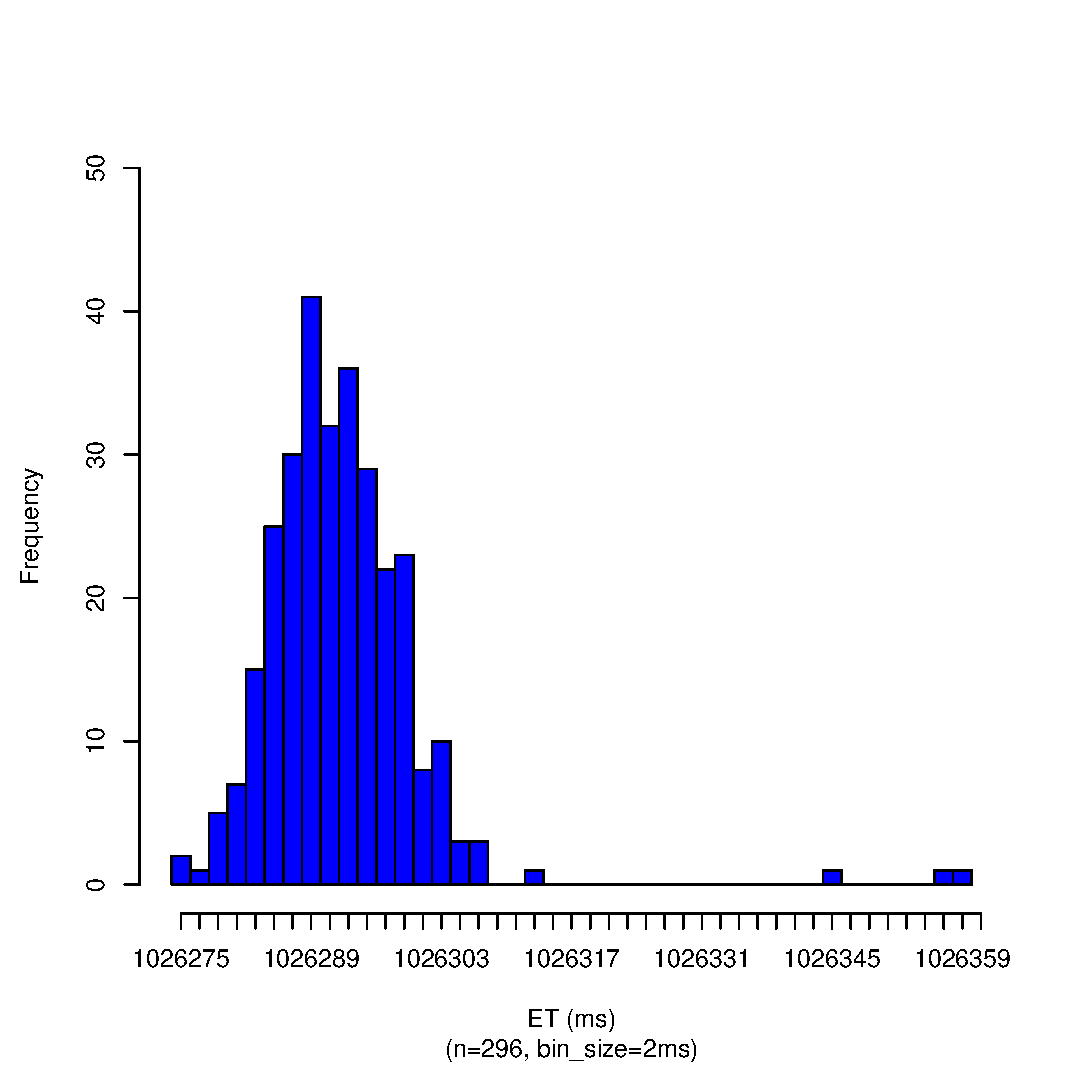
\includegraphics[scale=0.43]{1024_run/1024_sec_et_hist1.eps}
		\label{fig:inc1024_run1_et}
	}
	\subfigure[ET frequency on INC1024-Run2]{
		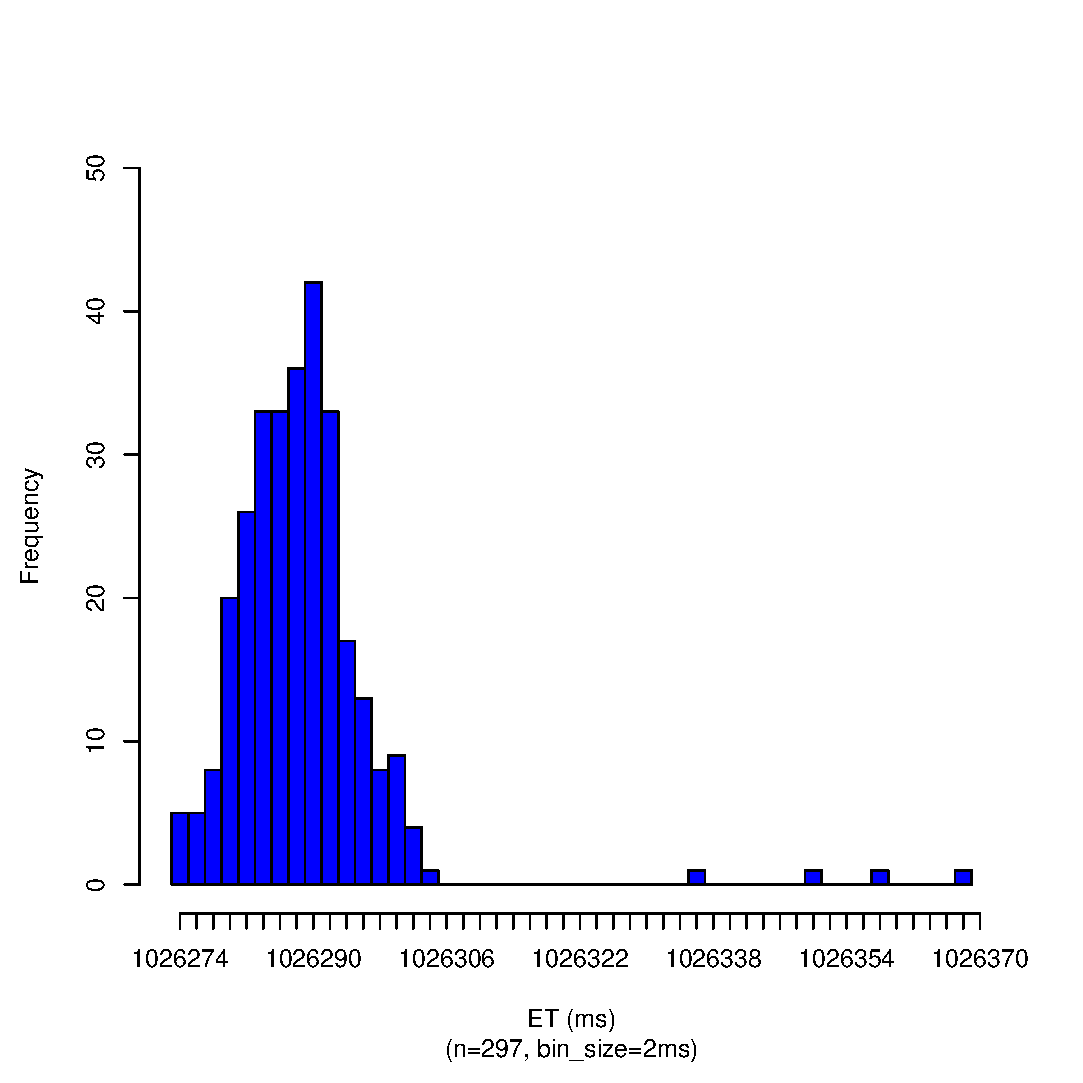
\includegraphics[scale=0.43]{1024_run/1024_sec_et_hist2.eps}
		\label{fig:inc1024_run2_et}
	}
	\subfigure[ET frequency on INC1024-Run3]{
		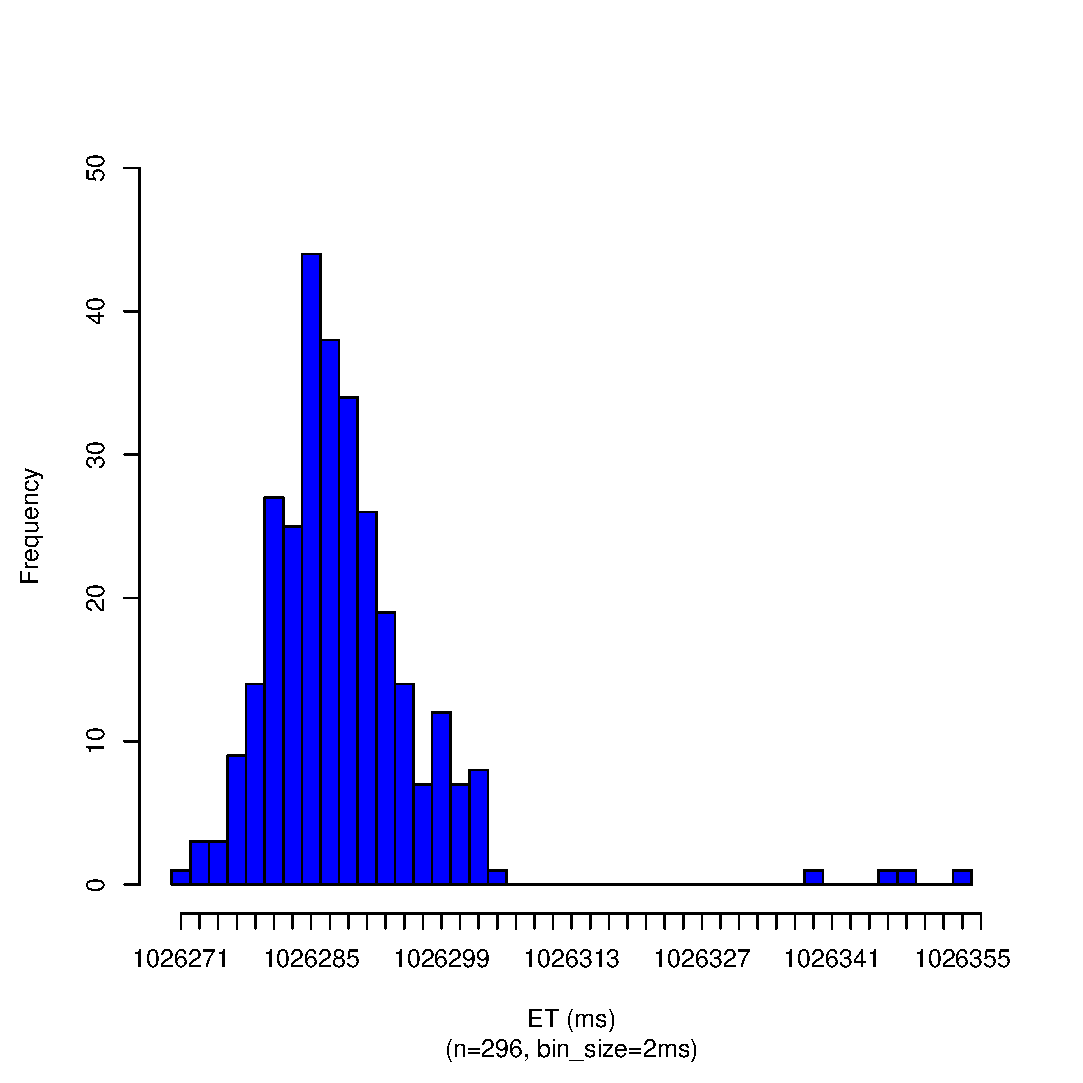
\includegraphics[scale=0.43]{1024_run/1024_sec_et_hist3.eps}
		\label{fig:inc1024_run3_et}
	}
	\caption{ET Histograms of Three Consecutive INC1024 Runs\label{fig:s9_inc1024_et}}
\end{figure}

\vspace\fill
\clearpage

\subsection{PT}

\begin{figure}[hp!]
	\centering
	\subfigure[PT frequency on INC1024-Run1]{
		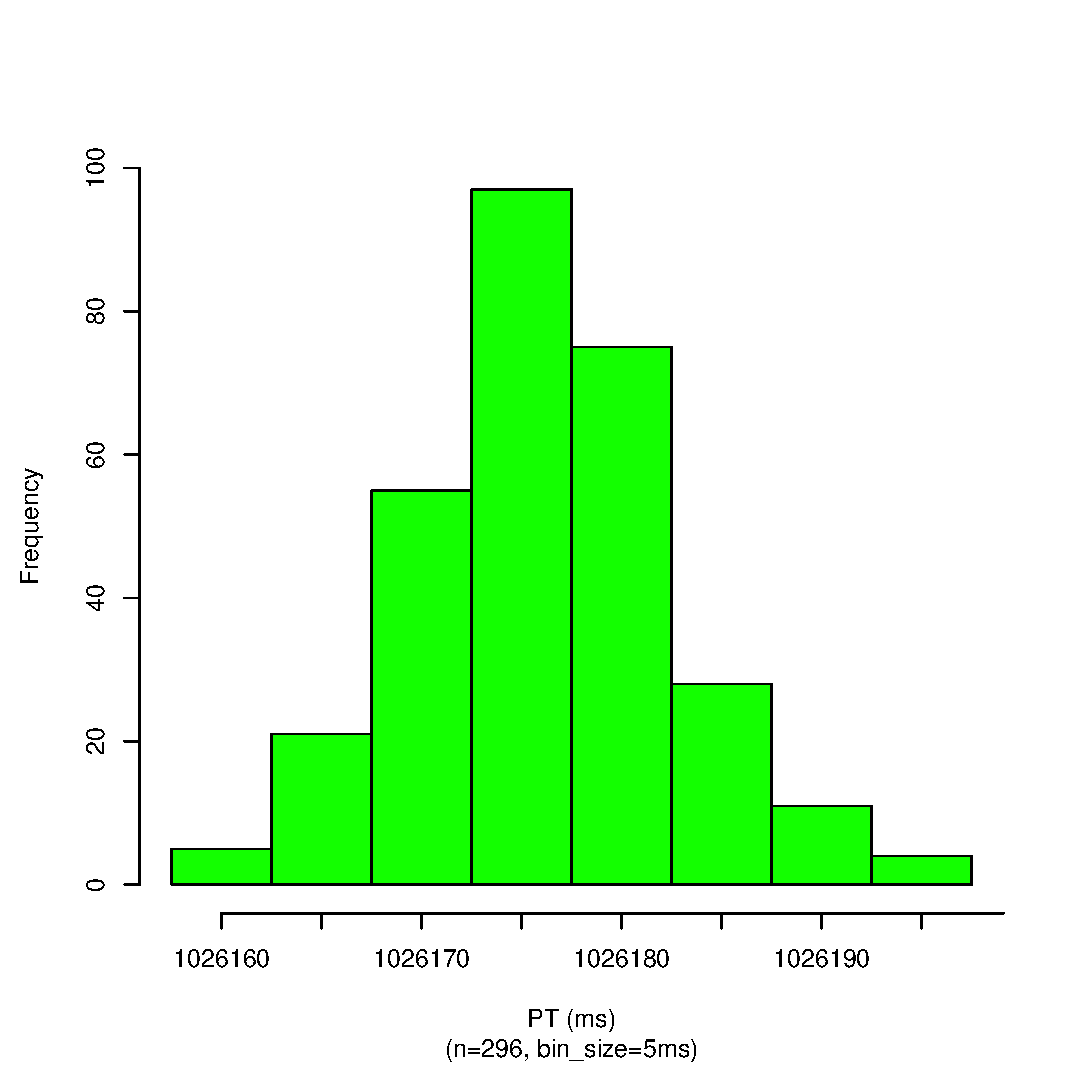
\includegraphics[scale=0.43]{1024_run/1024_sec_pt_hist1.eps}
		\label{fig:inc1024_run1_pt}
	}
	\subfigure[PT frequency on INC1024-Run2]{
		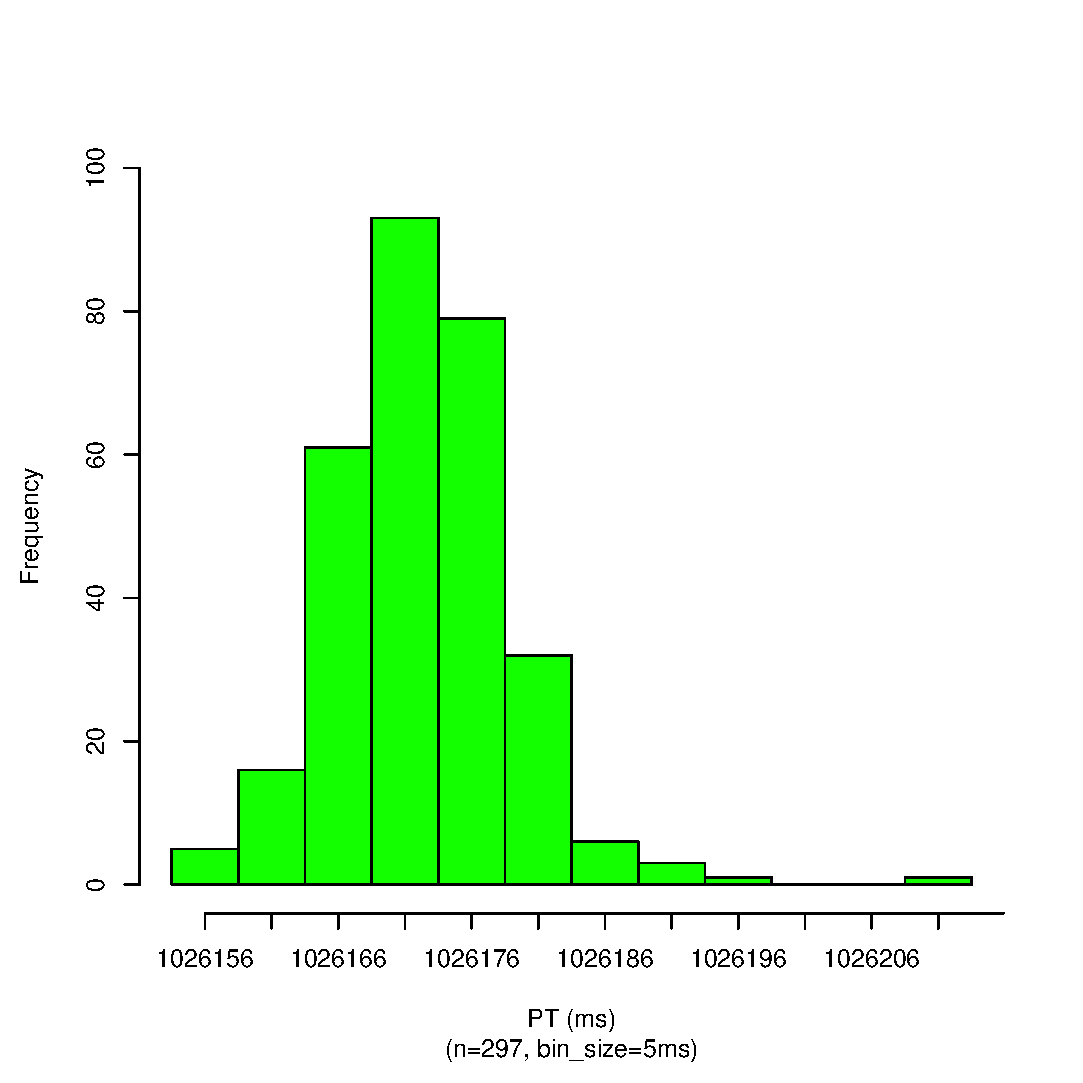
\includegraphics[scale=0.43]{1024_run/1024_sec_pt_hist2.eps}
		\label{fig:inc1024_run2_pt}
	}
	\subfigure[PT frequency on INC1024-Run3]{
		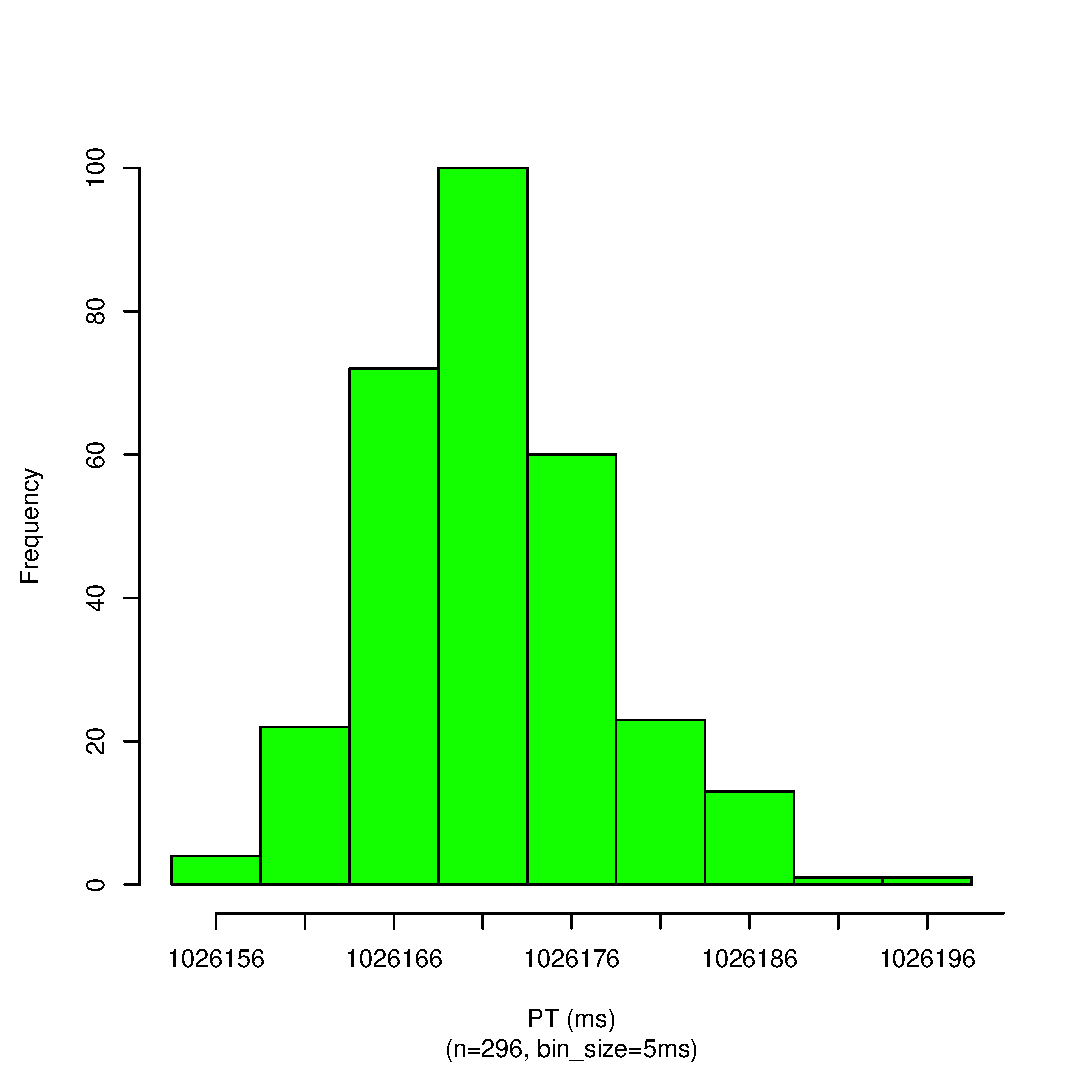
\includegraphics[scale=0.43]{1024_run/1024_sec_pt_hist3.eps}
		\label{fig:inc1024_run3_pt}
	}
	\caption{PT Histograms of Three Consecutive INC1024 Runs\label{fig:s9_inc1024_pt}}
\end{figure}
